\chapter{Алгоритмические и вычислительные аспекты}\label{sec:algo}

    В настоящей главе рассматриваются некоторые прикладные вопросы, связанные с правильными семействами:
    \begin{itemize}
        \item в разделе~\ref{sec:fpe} предлагается к рассмотрению один алгоритм шифрования, сохраняющего формат, основанный на сдвиговых преобразованиях в квазигруппах, порожденных правильными семействами булевых функций;
        \item раздел~\ref{sec:fastproper} посвящен рассмотрению одного улучшения \textquote{наивного} алгоритма распознавания правильности;
        %\item в разделе~\ref{sec:representatives} приводится один алгоритм построения системы представителей относительно действия группы изометрий (см. раздел~\ref{sec:proper_automorph}),
        \item в разделе~\ref{sec:experimental} приведены результаты численных экспериментов (количество булевых правильных семейств в некоторых классах, число ассоциативных троек).
    \end{itemize}

    Результаты главы ранее были опубликованы в~\cite{fpe22, sibecrypt23, tsar24}.


\section{Шифрование, сохраняющее формат}
\label{sec:fpe}
    Шифрование, сохраняющее формат (FPE, Format preserving encryption~\cite{bellare2009format}, далее $\fpe$-схема)~--- алгоритм, позволяющий зашифровывать сообщения из произвольного конечного множества $\Dom$ таким образом, что результат зашифрования также лежит в множестве $\Dom$.
    Такой тип алгоритмов довольно востребован на практике, о чем свидетельствует большое количество статей и предложений, рассматривающих стойкость таких криптомеханизмов (см., например,~\cite{bellare2009format, lee2015format, NIST16}).
    При этом подобные алгоритмы часто подвергаются специфическим атакам, связанным, в том числе, и с возможным относительно малым размером области определения (см., например,~\cite{hoang2018curse, amon2021three}).
    Известны \textquote{доказуемо стойкие} (о теоретико-сложностных сведениях/\textquote{доказуемой стойкости} см., например,~\cite{katz2020introduction}) алгоритмы как для очень малых ($ \lvert \Dom \rvert \approx 2^{10}$), так и для очень больших областей определения (размер которых приближается к размеру области определения стандартных блочных шифров, либо превышает их, см. т.н. wide-block encryption), в то время как для \textquote{средних} областей определения всё ещё не существует одного предпочтительного подхода.
    В этом разделе мы рассмотрим один возможный подход к построению $\fpe$-схем, основанный на квазигрупповых операциях.

\subsection{Общее описание $\fpe$-схем}
    $\fpe$-схемы позволяют зашифровывать тексты с заданным форматом (например, 6 десятичных цифр, номер кредитной карты, СНИЛС и так далее) таким образом, чтобы зашифрованное сообщение имело бы тот же формат, что и исходное. 
    Указанное свойство желательно, например, при шифровании баз данных, где поля записей имеют строго предписанный формат.
    Формализация данного требования выглядит следующим образом.
    \begin{definition}
        $\fpe$-схема~--- это тройка (вероятностных) алгоритмов $(\gen, \enc, \dec)$:
        \begin{itemize}
            \item (вероятностный) алгоритм генерации ключа $\gen$: на вход принимает пустую строку и возвращает ключ $K \in \Keys$;
            \item (детерминированный) алгоритм зашифрования $\enc$: на вход принимает ключ $K$, параметр-настройку $t \in \Twk$ и сообщение $m \in \Dom$ и возвращает шифртекст $ct \in \Dom$:
            \[
                \enc : \Keys \times \Twk \times \Dom \to \Dom;
            \]
            \item (детерминированный) алгоритм расшифрования $\dec$: на вход принимает ключ $K$, параметр-настройку $t \in \Twk$ и шифртекст $ct \in \Dom$ и возвращает открытый текст-сообщение $m \in \Dom$:
            \[
                \dec : \Keys \times \Twk \times \Dom \to \Dom.
            \]
        \end{itemize}
        Для указанной тройки алгоритмов должно выполняться требование корректности расшифрования: для любого ключа $K$, порождаемого алгоритмом $\gen$ и любых $t \in \Twk$, $m \in \Dom$ выполнено равенство
        \[
            \dec_K^t(\enc_K^t(m)) = m.
        \] 
    \end{definition}

    \begin{remark}
        Чаще всего алгоритм $\gen$ порождает равномерное распределение на множестве всех двоичных наборов длины $klen$.
        Далее мы будем опускать обозначение $\gen$ и предполагать, что ключ выбирается случайно равновероятно из множества $\{0, 1\}^{klen}$: $K \sample \{0, 1\}^{klen}$.
    \end{remark}
        
    \begin{remark}
        Введение дополнительного параметра-настройки $t \in \Twk$ обусловлено тем, что область определения $\Dom$ может быть слишком маленькой, что приведет к возможности атаки по словарю/кодовой книге, в ходе которой противник получает шифртексты для всех возможных сообщений $m \in \Dom$ и может далее осуществлять бесключевое чтение.
    \end{remark}

    \begin{remark}
        Множество $\Dom$ может быть устроено нестандартно. 
        К примеру, если необходимо шифровать номера банковских карточек, то на множество $\Dom$ налагаются следующие ограничения:
        \begin{itemize}
            \item формат номера~---~16 десятичных цифр;
            \item первые 6 цифр кодируют $ID$ банка, выдавшего карточку (для многих приложений они должны храниться в открытом виде);
            \item последняя цифра является контрольной суммой и не должна зашифровываться.
        \end{itemize} 
        Таким образом, необходимо зашифровывать 9 средних цифр в номере карточки, в этом случае мы имеем:
        \[
            \Dom = \{0, \ldots 9 \}^{9}, \quad \lvert \Dom \rvert \approx 2^{30}.
        \]
    \end{remark}

    \textquote{Обычный} блочный шифр действует на множестве двоичных строк фиксированной длины (например, $\Dom = \{0, 1\}^{128}$ для алгоритма \textquote{Кузнечик}, см.~\cite{kuzn}), и результат шифрования элемента $m \in \Dom$ может оказаться вне требуемого множества: $\enc_K^t(m) \not\in \Dom$.
    В связи с этим актуальна задача разработки алгоритма, который по ключу $K$ и параметру $t$ порождал бы некоторую подстановку $\enc_K^t \in \SSS_{\Dom}$ со следующими желательными свойствами:
    \begin{itemize}
        \item операции $\enc_K^t$, $\dec_K^{t}$ быстро вычислимы;
        \item при случайном выборе ключа $K \sample \gen$ получаемое отображение $\enc_K^t(\cdot)$ вычислительно неотличимо (более подробно о понятии вычислительной неотличимости см.~\cite{katz2020introduction}) от случайной подстановки $\pi \sample \SSS_{\Dom}$; 
        \item вероятность успешной атаки схемы мала даже для малых ($\lvert \Dom \rvert \approx 2^{20}$ и менее) областей определения.
    \end{itemize}

\subsection{Подход на основе квазигрупп}
    В работе~\cite{fpe22} был предложен подход на основе квазигрупповых операций сдвига.
    В качестве базовой сложной задачи предлагается рассматривать задачу различения случайной подстановки от структурированной: пусть дана некоторая квазигруппа $Q$, и мы хотим измерить, насколько композиция квазигрупповых операций (например, серия умножений слева на случайные элементы квазигруппы) похожа на случайную подстановку на множестве $Q$.

\subsubsection{Базовая задача}

    Задачи изучения неотличимости случайной подстановки от структурированной в несколько неформальном модельном описании может быть представлена следующим образом (больше о теоретико-сложностных сведениях в контексте изучения криптографических механизмов и протоколов можно посмотреть, например, в~\cite{katz2020introduction}).
    \begin{enumerate}
        \item Противник $\mathcal{A}$ (вероятностный алгоритм) взаимодействует с оракулом $\mathcal{O}$, реализующим некоторую функцию $f$.
        Перед началом взаимодействия оракул \textquote{подбрасывает монетку} (выбирает случайно равновероятно бит $b \sample \{0, 1\}$).
        \begin{itemize}
            \item если бит $b = 0$, оракул выбирает случайную подстановку $\pi \sample \SSS_Q$ на множестве $Q$, и при дальнейших запросах к нему от противника $\mathcal{A}$ вычисляет функцию $f$ по правилу $f(x) = \pi(x)$;
            \item если бит $b = 1$, оракул выбирает $\lambda$ случайных элементов $q_i \sample Q$, $i = 1, \ldots, \lambda$ и при дальнейших запросах к нему от противника $\mathcal{A}$ вычисляет функцию $f$ по правилу
            \begin{equation}
            \label{eq:structured}
                f(x) = L_{q_1} \left( L_{q_2} \left( \ldots L_{q_{\lambda}}(x) \ldots \right) \right).
            \end{equation}
        \end{itemize}
        \item На запросы $x$ противника $\mathcal{A}$ оракул $\mathcal{O}$ возвращает ответ $f(x)$.
        \item Изучая ответы оракула, противник должен понять, какой бит был выбран оракулом до начала взаимодействия, то есть по какому правилу оракул вычисляет функцию $f$.
        %Вероятность успешного угадывания противником секретного значения $b$ может быть оценена сверху как функция от параметров \textquote{количество запросов к оракулу} и \textquote{количество тактов вычислений противника}.
    \end{enumerate}
    Параметрами рассматриваемой модели, от которых зависит успешность угадывания противником секретного значения $b$ являются \textquote{количество запросов к оракулу} и \textquote{время работы противника} (количество тактов вычислений).
    Если противник может с высокой вероятностью и низкой затратой рассматриваемых ресурсов правильно угадывать значение бита $b$, то он способен отличать истинно случайную подстановку $\pi \in \SSS_Q$ от \textquote{структурированной} 
    \[
        f(x) = L_{q_1} \left( L_{q_2} \left( \ldots L_{q_{\lambda}}(x) \ldots \right) \right).
    \]

    Вероятность успеха противника зависит от структуры используемой квазигруппы. 
    Так, например, если рассмотреть в качестве базовой квазигруппу $(Q, \circ) = (\ZZ_{2^n}, +)$, то полученная структурированная подстановка будет тривиально отличима от случайной, поскольку в таком случае \textquote{левым умножением} является сложение поданного на вход элемента со случайными элементами $L_q(x) = q + x$, и полученное преобразование будет аффинным; в частности, с вероятностью 1 будет выполнено равенство:
    \[
        f(x + y) - f(x) = y,
    \]
    что позволит легко отличить его от случайной подстановки.

    В контексте рассматриваемой $\fpe$-схемы можно выделить следующие важные свойства квазигруппы, которые могут потенциально усложнять криптоанализ, а значит, делать схему более стойкой (отметим также, что выделенные свойства упоминаются, например, в~\cite{EdonR} как необходимые при использовании квазигрупп в криптографических механизмах).
    \begin{enumerate}
        \item Малый индекс ассоциативности квазигруппы $Q$ (см. раздел~\ref{subsec:assoc_problem}): если в квазигруппе $Q$ большое количество ассоциативных троек, то в операции~(\ref{eq:structured}) реальное количество элементов, на которых умножается $m$, может быть сильно меньше, чем $\lambda$.
        \item Полиномиальная полнота квазигруппы $Q$ (см. раздел~\ref{sec:polycompleteness}): свидетельством в пользу того, что рассматриваемая задача может быть сложной, является $\mathsf{NP}$-полнота задачи проверки разрешимости уравнений над полиномиально полной квазигруппой общего вида.
        Тем не менее, такое наблюдение может давать теоретические гарантии лишь в <<худшем>> случае, ничего не говоря о <<генерической>> сложности задачи~\cite{kapovich2003generic}.
        \item Отсутствие подквазигрупп в квазигруппе $Q$ (см. раздел~\ref{sec:subquasi}): если в $Q$ имеются достаточно большие подквазигруппы, и исходный элемент $m$ принадлежал такой подквазигруппе, то операция~(\ref{eq:structured}) может сохранять принадлежность элемента $m$ подквазигруппе, что дает критерий на отличимость случайной подстановки от структурированной и может рассматриваться как потенциальная слабость алгоритма.
    \end{enumerate}
    
    Отметим также, что $L$-сдвиги (и им родственные преобразования) рассматривались, в частности, в работах~\cite{markovski2017quasigroup, artamonov18, yash22}.
    Так, в работе~\cite{yash22} среди прочего показано, что для любой квазигрупповой операции $\circ$ при случайном независимом выборе элементов $q_i \in \Dom$ (при условии, что носитель распределения $q_i$ достаточно большой) распределение элемента $ct$ экспоненциально быстро (при увеличении параметра $\lambda$) сходится к равновероятному распределению на множестве $\Dom$.
    При этом результаты работы~\cite{yash22}, вообще говоря, не применимы к ситуации, в которой противник может получать образы различных адаптивно выбираемых $m$ (см. постановку задачи выше), но могут свидетельствовать в пользу сложности рассматриваемой задачи для некоторых квазигрупп.

\subsubsection{Предлагаемая $\fpe$-схема}
\label{sec:fpescheme_concrete}

    Для того, чтобы получить $\fpe$-схему на основе описанной выше задачи, необходимо задать пару алгоритмов $(\enc, \dec)$~--- отображений из $\Keys \times \Twk \times \Dom$ в $\Dom$.
    В работе~\cite{fpe22} был предложен следующий подход.
    Для зашифрования элемента $m$ на ключе $K$ и параметре $t$ выполним следующие шаги.
    \begin{enumerate}
        \item По ключу $K \in \Keys$ и параметру $t \in \Twk$ построим с помощью псевдослучайной функции (см., например, функцию $\mathsf{PRF}$ из работы~\cite{alekseev16}) последовательность псевдослучайных элементов $q_1, \ldots, q_{\lambda} \in Q$.
        \item Переведем с помощью левых квазигрупповых сдвигов заданный элемент $m \in \Dom$ в элемент
        \[
            ct = L_{q_1} \left( L_{q_2} \left( \ldots L_{q_{\lambda}}(m) \ldots \right) \right).
        \]
    \end{enumerate}
    Для расшифрования сообщения $ct$ сначала получим согласно п.~1 элементы $q_1, \ldots, q_{\lambda} \in Q$, а затем последовательно решим уравнения вида $q_i \circ x = y_i$ ($\lambda$ штук) и получим решение $m$.

    Сложность нахождения решения $m$ по заданным $(t, ct)$ и неизвестному $K$ в предложенной схеме обуславливается двумя факторами (см. более подробное доказательство в~\cite{fpe22}).
    \begin{enumerate}
        \item По известному $t$ и неизвестному $K$ трудно восстановить элементы $q_1, \ldots, q_{\lambda} \in Q$, полученные в п.~1 с помощью псевдослучайной функции (и даже отличить их от истинно случайных).
        \item При неизвестных $q_1, \ldots, q_{\lambda}$ трудно отличить результат применения структурированной подстановки 
        \[
            x \to L_{q_1} \circ (L_{q_2} \circ \ldots \circ (L_{q_{\lambda}} \circ x) \ldots )
        \]
        от результата применения случайной подстановки
        \[
            x \to \pi(x).
        \]
    \end{enumerate}

    Рассмотрим ограниченный класс квазигрупп, порожденных правильными семействами функций.
    Пусть $\ff$, $\gf$~--- два правильных семейства размера $n$ на прямом произведении $H^n$ групп $(H, +)$ (не обязательно абелевых).
    Как было отмечено выше (см. раздел~\ref{sec:assoctriples_proper}), операция умножения $\circ \colon H^n \times H^n \to H^n$, определяемая равенством
    \begin{equation}
    \label{eq:circ}
        \xx \circ \yy = \sigma_{\ff}(\xx) + \sigma_{\gf}(\yy),
    \end{equation}
    где $\sigma_{\ff}(\xx) = \xx + \ff(\xx)$ (см. определение~\ref{def:sprop}), а сложение $+$ понимается как покомпонентное сложение в группе $H^n$, задает структуру квазигруппы.

    Определенное таким образом умножение в $H^n$ может быть эффективно обращено используя следующее соображение.
    Рассмотрим подстановку $\sigma^{-1}_{\ff}$. 
    Как было отмечено в разделе~\ref{sec:properinverse}, подстановка $\sigma^{-1}_{\ff}$ также порождается некоторым правильным семейством $\widetilde{\ff}$ (которое было названо дуальным).
    Семейства $\ff$ и $\widetilde{\ff}$ связаны соотношением:
    \begin{equation}
        \label{eq:dual}
        \widetilde{\ff}(\xx) = (-\xx) + \sigma^{-1}_{\ff}(\xx), \quad \sigma_{\ff}(\xx) = \xx + \ff(\xx), \quad x \in H^n.
    \end{equation}

    Таким образом, если $\ff$ и $\widetilde{\ff}$~--- пара правильных семейств, связанных соотношением~(\ref{eq:dual}), и операция $\circ$ задается формулой~(\ref{eq:circ}), то операция $x \circ y$ обращается справа следующим образом:
    \[
        \xx = \sigma_{\widetilde{\ff}} \left( (\xx \circ \yy) - \sigma_{\gf}(\yy) \right).
    \]
    Аналогичным образом операция $\xx \circ \yy$ может быть обращена слева, используя <<дуальное>> к $\gf$ семейство $\widetilde{\gf}$.

    Из этих соображений вытекает, что как $L$-преобразование, так и обратное к нему $L^{-1}$ могут быть заданы с помощью правильных семейств функций, что позволяет перейти от табличного задания квазигруппы к функциональному.



\section{Алгоритм проверки правильности булевых семейств}
\label{sec:fastproper}

    В настоящем разделе мы рассмотрим один алгоритм проверки правильности булева семейства $\ff_n$, время работы которого существенно лучше \textquote{наивного} алгоритма.

\subsection{О сложности проверки правильности}
    Полученное в разделе~\ref{sec:uso} взаимно-однозначное соответствие между правильными семействами булевых функций и $\uso$-ориентациями позволяет перенести часть результатов из теории, развитой в работах~\cite{USOphd,USOcomplexity,numberUSO}, на правильные семейства. 
    В частности, верны следующие утверждения.

    \begin{corollary}[{\cite[теорема~5]{USOcomplexity}}]
    \label{coroll:conp}
        Пусть семейство булевых функций $\ff_n$ задано в виде схемы из функциональных элементов в некотором функционально полном конечном базисе. 
        Тогда задача распознавания правильности семейства по его схеме из функциональных элементов является $\mathsf{coNP}$-полной.
    \end{corollary}

    Заметим, что указанное выше утверждение для случая задания функций в виде КНФ было известно и ранее (см. работу~\cite{nosov98}).
    При этом в определенных случаях задача проверки правильности может быть упрощена, в частности, за счет вида графа существенной зависимости~\cite{rykov10, rykov14}.

    Таким образом, нахождение быстрого (полиномиального по размеру семейства $n$) алгоритма проверки правильности семейства представляется маловероятным.
    Заметим, что \textquote{наивный} алгоритм проверки правильности требует $4^n$ операций вычисления значения семейства $\ff_n$ на наборе $\xx \in \EE_2^n$.

\subsection{Описание алгоритма}
    Рассмотрим алгоритм проверки правильности со сложностью $2 \cdot 3^n$ операций вычисления семейства $\ff_n$ на наборе $x$, который является следствием теоремы~\ref{thm:self_proper}.
    На вход алгоритму подаётся семейство булевых функций $\ff_n$ (например, в виде схем из функциональных элементов в некотором базисе).
    Алгоритм перебирает все проекции исходного семейства $\ff_n$, проверяя выполнение свойства несамодвойственности на какой-либо \textbf{единственной паре} антиподальных наборов из области определения проекции.

    Если на выбранной паре антиподов свойство самодвойственности выполнено, то исходное семейство не может быть правильным: нашлась такая проекция, для которой принимаются противоположные значения, а значит, эта проекция (и исходное семейство) не является правильным семейством (см. замечание~\ref{rem:antipode}).

    Если на выбранной паре антиподов свойство самодвойственности не выполнено, то рассматриваемая проекция заведомо не является самодвойственным отображением.
    Поскольку в ходе работы алгоритма перебираются все возможные проекции семейства, то из теоремы~\ref{thm:self_proper} следует, что если семейство проходит проверки на несамодвойственность на всех проекциях, то оно является правильным.

    %Если существует такая проекция, для которой свойство самодвойственности выполнено, то алгоритм останавливает работу и выдаёт результат \textquote{семейство $\ff_n$ не является правильным}, поскольку в таком случае по лемме~\ref{lemma:dual} найдётся самодвойственная проекция $\ff_n$, а значит, $\ff_n$ не является правильным.

    %Если семейство $\ff_n$ проходит все проверки, то у нас есть гарантия, что для $\ff_n$ и всех его проекций не выполнено свойство самодвойственности: если бы существовал хотя бы один набор $\alpha$, для которого $\overline{F(\alpha)} = F(\bar{\alpha})$, то по лемме~\ref{lemma:dual} нашлась бы полностью самодвойственная проекция, что было исключено в ходе проверок.

    Таким образом, мы доказали корректность следующего алгоритма.

    \begin{Algo}
        Цикл по всем возможным наборам $\xx \in \EE_3^n$:
        \begin{enumerate}
            \item Построить два набора $\yy, \zz \in \EE_2^n$ по правилу:
            \begin{itemize}
                \item если $x_i \in \{0, 1\}$, то положить $y_i \gets x_i$, $z_i \gets x_i$;
                \item в противном случае положить 
                $y_i \gets 0$, $z_i \gets 1$.
            \end{itemize}
            \item Если существует номер $j$, что $y_j \ne z_j$, и $f_j(y) \ne f_j(z)$, вернуть ответ: \textquote{$\ff_n$ не является правильным}.
        \end{enumerate}
        Если все проверки пройдены успешно, то вернуть: \textquote{$\ff_n$ является правильным}.
    \end{Algo}

    Рассмотренный алгоритм позволяет снизить количество вычислений значения отображения $\ff_n$ в точке с $4^n$ до $2 \cdot 3^n$.
    Вопрос о возможном обобщении алгоритма со случая $k = 2$ на логики большей значности пока что остаётся открытым.


% \section{Алгоритм построения представителей}
% \label{sec:representatives}

%     Описанное в разделе~\ref{sec:isometry_proper} действие группы $\GGG$ на множестве правильных семейств позволяет говорить об отношении эквивалентности между правильными семействами.
%     \begin{definition}
%         Два семейства $\ff_n$ и $\gf_n$ на $\EE_k^n$ назовем эквивалентными, если существует пара изометрий 
%         \[
%             \Phi, \Psi \in Iso(\EE_k^n)
%         \]
%         таких, что $\gf_n(\xx) = \Phi(\ff_n(\Psi(\xx)))$.
%     \end{definition}
%     Таким образом можно говорить о классах эквивалентности семейств, а также о системе представителей для всех семейств размера $n$.

% \subsection{Вспомогательные утверждения}

%     Предварительно докажем несколько дополнительных свойств.

%     \begin{lemma}
%         Пусть $\ff_n$~--- правильное семейство.
%         Тогда найдется такая точка $\xx$, что в локальном графе взаимодействий $G_{\ff}(\xx)$ существует сток.
%     \end{lemma}

%     \begin{proof}
%         \TODO{пока что без доказательства, но это точно верно}

%         \TODO{Это только для $\EE_2^n$ или для всех?}
%     \end{proof}

    % \begin{proof}
    %     Докажем от противного.
    %     Пусть для каждой точки $x$ граф $Gf(x)$ не содержит стоков. %является ациклическим.
    %     Выберем такую точку $x$, что цикл в графе $Gf(x)$ является кратчайшим среди всех возможных: 
    %     \[
    %         i_1 \to i_2 \to \ldots \to i_k \to i_1.
    %     \]
    %     Рассмотрим ограничение $g$ семейства $f$ на подпространство $L = \langle e_{i_1}, \ldots, e_{i_k} \rangle$.
    %     Относительно $g$ мы можем утверждать, что:
    %     \begin{itemize}
    %         \item $g$~--- правильное семейство размера $k$;
    %         \item для \textbf{каждой} точки $x$ граф $Gg(x)$ является либо циклом длины ровно $k$, либо состоит из $k$ несвязных вершин.
    %     \end{itemize}
    %     Второе утверждение следует из того факта, что $Gg(x)$~--- подграф $Gf(x)$ для каждой точки $x$, а потому не может содержать цикл длины меньшей чем $k$.
    %     При этом $Gg(x)$ также не может содержать и нескольких циклов длины $k$ (в противном случае мы могли бы <<укоротить>> исходный цикл).
    %     Случай несвязных вершин
    %     Другими словами, матрица <<локальной существенной зависимости>> для каждой точки $x$ является перестановочной матрицей (возможно, разной). 
    %     Покажем, что такая ситуация невозможна для правильных семейств.

    %     Рассмотрим точку $x = (0, \ldots, 0)$, пусть значение $f(x) = \alpha$.
    %     Будем покоординатно переходить от точки $x$ к ее антиподу, при этом следя за тем, как меняется значение функции.

    %     Зададим $e_{i_0} = (1, 0, \ldots, 0)$, $i_0 = 1$.
    %     Рассмотрим точку $x \oplus e_{i_0}$.
    %     Поскольку $Gg(x)$~--- цикл, то при переходе к указанной точке \textbf{ровно одна} из координат функции изменится, пусть это будет $i_1$ (в силу того, что $Gg(x)$~--- простой цикл).
    %     Заметим, что $i_1 \ne i_0$ (или, другими словами, $i_i \not \in \{i_0\}$), поскольку иначе $g_{i_0}$ существенно зависит от $x_{i_0}$.
    %     В указанной точке значение функции будет равно 
    %     \[
    %         g(x \oplus e_{i_0}) = \alpha \oplus e_{i_1}.
    %     \]
    %     Далее перейдем от $x \oplus e_{i_0}$ к точке $x \oplus e_{i_0} \oplus e_{i_1}$.
    %     При этом поменяется функция с индексом $i_2$.

    %     Будем продолжать указанный процесс.
    %     На каждом шаге будет меняться ровно одна координата функции.
    %     Покажем, что на каждом шаге мы будем получать координату, которая не встречалась ранее, т.е. на $j$-м шаге имеем 
    %     \[
    %         i_{j+1} \not \in \{i_0, \ldots, i_j \}.
    %     \]
    %     Предположим противное: $i_{j+1} = i_k$.
    %     Тогда рассмотрим следующие точки:
    %     \[
    %         u = x \oplus e_{i_0} \oplus \ldots \oplus e_{i_{k-1}},
    %     \]
    %     \[
    %         v = x \oplus e_{i_0} \oplus \ldots \oplus e_{i_{j}} = u \oplus e_{i_k} \oplus \ldots \oplus e_{i_{j}}.
    %     \]
    %     Пусть
    %     \[
    %         g(u) = \beta = \alpha \oplus e_{i_1} \oplus \ldots \oplus e_{i_{k}},
    %     \]
    %     тогда по определению координат $i$ имеем 
    %     \begin{equation*}
    %         g(v) = \beta \oplus e_{i_{k+1}} \oplus \ldots \oplus e_{i_j} \oplus e_{i_{j+1}} = \\
    %         = \beta \oplus e_{i_{k}} \oplus \ldots \oplus e_{i_j} \oplus e_{i_{j}}.
    %     \end{equation*}
    %     Тогда точки $u$ и $v$ различаются в координатах $i_k, \ldots, i_j$, и в тех же координатах различны и значения функции $g(u)$ и $g(v)$, что противоречит правильности $g$.

    %     Таким образом, мы имеем следующий результат: на каждом шаге можно менять одну из координат текущей точки, при этом будет меняться координата функции, причем координаты не повторяются.

    %     Следовательно, в конечном счете мы дойдем до антипода $y$ точки $x$, и $g(x)$ будет отличаться от $g(y)$ во всех координатах, что также противоречит правильности.
    %     Мы пришли к противоречию, следовательно, исходная предпосылка была неверна.
    % \end{proof}

%     \begin{corollary}
%         Если $\ff$~--- правильное семейство, то существует такая точка $\uu$ и такой индекс $j$, что справедливо равенство 
%         \[
%             \ff(\xx) = \ff(\xx \oplus e_j).
%         \]
%     \end{corollary}

%     \begin{proof}
%         Достаточно рассмотреть точку $\xx$, в которой $\ff$ локально постоянно по направлению $e_j$.
%     \end{proof}

%     \begin{corollary}
%         \label{corol:stdform}
%         Если $\ff$~--- правильное семейство, то существует эквивалентное правильное семейство $\gf \equiv \ff$ со свойством
%         \[
%             \gf(0, \ldots, 0, 0) = \gf(0, \ldots, 0, 1) = (0, \ldots, 0, 0)^T.
%         \]
%     \end{corollary}

%     \begin{proof}
%         Возьмем точку $\uu$ из предыдущего утверждения.
%         Рассмотрим первое эквивалентное семейство $\gf^{1}(\xx) = \ff(\xx \oplus \uu)$ (внутренний сдвиг).
%         Затем перейдем ко второму эквивалентному путем перенумерации функций и переменных так, чтобы $j$ перешло в $n$.
%         Затем сдвинем всё семейство (внешний сдвиг) так, чтобы оба значения были равны нулю.
%     \end{proof}


% \subsection{Алгоритм построения представителей}

%     Покажем, что \textbf{систему представителей} правильных семейств размера $n+1$ относительно действия \textbf{полной группы} 
%     \[
%         \underbrace{\ZZ_2^n}_{\text{внутр. сдвиг}} \times \underbrace{\ZZ_2^n}_{\text{внеш. сдвиг}} \times \underbrace{\SSS_n}_{\text{согл. перенум.}}
%     \]
%     можно построить из \textbf{системы представителей} правильных семейств размера $n$ относительно действия \textbf{неполной группы} 
%     \[
%         \underbrace{\ZZ_2^n}_{\text{внеш. сдвиг}} \times \underbrace{\SSS_n}_{\text{согл. перенум.}}.
%     \]
%     Покажем это.
%     Сначала мы можем перейти от произвольного семейства $\widetilde{\ff_{n+1}}$ к эквивалентному ему семейству $\ff_{n+1}$ со свойством, указанном в следствии~\ref{corol:stdform} (действие полной группы).
%     Рассмотрим разложение семейства $\ff$ размера $n+1$ на два семейства размера $n$:
%     \[
%         \ff_{n+1}(\xx, x_{n+1}) = 
%         \begin{bmatrix}
%             x_{n+1} \cdot \ff_n^1(\xx) \oplus \overline{x_{n+1}} \cdot \ff_n^0(\xx) \\
%             f(\xx)
%         \end{bmatrix} = 
%         \begin{bmatrix}
%             x_{n+1} \cdot \gf(\xx) \oplus \overline{x_{n+1}} \cdot \hf(\xx) \\
%             f(\xx)
%         \end{bmatrix},
%     \]
%     где $\xx = (x_1, \ldots, x_n)$.
%     Поскольку $\ff_{n+1}$ выбрано в соответствии со следствием~\ref{corol:stdform}, то для $\gf$ и $\hf$ справедливы равенства:
%     \[
%         \gf(0, \ldots, 0) = \hf(0, \ldots, 0) = (0, \ldots, 0)^T.
%     \]
%     Таким образом, $\gf$ и $\hf$~--- \textquote{несдвинутые} правильные семейства размера $n$.
%     Для каждого из них существует представитель (относительно действия неполной группы) размера $n$, отличающийся, возможно, применением согласованной перестановки (не может отличаться внешним сдвигом, т.к. представители несдвинутые):
%     \[
%         \gf(\xx) = \sigma_1(\gf)(\xx), \quad \hf(\xx) = \sigma_2(\hf)(x).
%     \]
%     Рассмотрим эквивалентное $\ff_{n+1}$ семейство: согласованно перенумеруем первые $n$ функций и координат в соответствии с подстановкой $\sigma^{-1}$.
%     Обозначим $\tau = \sigma_1^{-1} \circ \sigma_2$.
%     Тогда семейство
%     \[
%         \begin{bmatrix}
%             x_{n+1} \cdot \gf(\xx) \oplus \overline{x_{n+1}} \cdot \tau(\hf)(\xx) \\
%             f'(\xx)
%         \end{bmatrix}
%     \]
%     будет эквивалентно семейству $\ff_{n+1}$ (относительно действия полной группы).

%     Таким образом, мы смогли из представителей $\gf$ и $\hf$ размера $n$ получить представителя $\ff_{n+1}$ размера $n+1$ для любого семейства размера $n+1$.
%     Полученное множество представителей можно расширить (путем применения внешних, внутренних сдвигов и перестановок) до полного набора правильных семейств.
%     Заметим, что построенное множество представителей может быть избыточно в том смысле, что некоторые из полученных представителей на самом деле могут оказаться эквивалентными.

%     Таким образом, можно предложить следующий алгоритм построения представителей размера $n+1$.
%     \begin{Algo}
%         Пусть задано система представителей $\mathcal{A}$ размера $n$ относительно действия неполной группы (внешних сдвигов + согласованных перенумераций).
%         Для построения системы представителей размера $n+1$ относительно действия группы необходимо выполнить следующие действия:
%         \begin{enumerate}
%             \item выбрать $\gf, \hf \in \mathcal{A}$;
%             \item выбрать $\tau \in \SSS_n$;
%             \item построить граф смежности для пары правильных семейств $(\gf(\xx), \tau(\hf)(\xx))$ аналогично тому, как это сделано в алгоритме из работы~\cite{galatenko2022generation};
%             \item задать $(n+1)$-ю функцию $f_{n+1}$ на компонентах связности полученного графа всеми возможными способами;
%             \item для каждого полученного продолжения $f_{n+1}$ построить представителя (относительно действия полной группы)
%             \[
%                 \begin{bmatrix}
%                     x_{n+1} \cdot \gf(\xx) \oplus \overline{x_{n+1}} \cdot \tau(\hf)(\xx) \\
%                     f_{n+1}(\xx)
%                 \end{bmatrix}.
%             \]
%         \end{enumerate}
%     \end{Algo}

%     \TODO{Написать о том, насколько сильно ускоряется перебор? Или зачем это всё}



\section{Некоторые результаты численных экспериментов}
\label{sec:experimental}

    В разделе~\ref{sec:fpe} был описан один подход к построению алгоритма шифрования, сохраняющего формат сообщений, предложена к рассмотрению одна конкретная конструкция на основе правильных семейств функций, а также выделены три основных свойства, которые можно предъявлять к квазигруппам, которые потенциально могут быть использованы в рассмотренном алгоритме: малое число ассоциативных троек, полиномиальная полнота, отсутствие (больших) подквазигрупп.

    В настоящем разделе мы приведем некоторые результаты численных экспериментов:
    \begin{itemize}
        \item в разделе~\ref{sec:numproper} приводятся точные значения числа булевых правильных семейств малых размеров;
        \item раздел~\ref{sec:assoc_index_proper} посвящен вычислению индексов ассоциативности для квазигрупп, порожденных парами правильных семейств булевых функций; 
        \item в разделе~\ref{sec:subquasi_polycomplete} рассматриваются результаты изучения свойств простоты и аффинности в квазигруппах, порожденных парами правильных семейств булевых функций.
    \end{itemize}


\subsection{Число различных булевых правильных семейств}
\label{sec:numproper}

    В разделе~\ref{sec:fastproper} был предложен алгоритм, который позволяет ускорить проверку правильности семейства.
    С использованием указанного алгоритма оказывается возможным вычисление точного значения числа правильных семейств в различных классах.
    Введем следующие обозначения.
    \begin{itemize}
        \item $\Delta(n)$: число булевых треугольных семейств размера $n$;
        \item $\Delta^{\loc}(n)$: число булевых локально-треугольных семейств размера $n$;
        \item $\Delta^{\rec}(n)$: число булевых рекурсивно-треугольных семейств размера $n$;
        \item $T(n)$: число булевых правильных семейств размера $n$.
    \end{itemize}

    Соберем известные результаты для числа правильных булевых семейств различных классов и размеров (см. таблицу~\ref{tab:countfamilies}).
    Число треугольных семейства размера $n=5$ получено в работе~\cite{allen2014counting} (число $CP$-сетей размера $n=5$).
    Число правильных семейств размера $n=5$ получено в работе~\cite{mathew2013enumerating} (для числа классов эквивалентности замощений пространства), а также в работах~\cite{bosshard2017pseudo, USOphd} (для числа одностоковых ориентаций).
    Число $\Delta^{\loc}(5)$ на настоящий момент неизвестно.

    \begin{table}[h]
        \centering
        \captionsetup{justification=centering} % выравнивание подписи по-центру
        \caption{\label{tab:countfamilies} Число треугольных, рекурсивно треугольных, локально треугольных и правильных булевых семейств размера $n$.}
        \begin{tabular}{|c|c|c|c|c|}
            \toprule
            Размер $n$  & $\Delta(n)$ & $\Delta^{\rec}(n)$ & $\Delta^{\loc}(n)$ & $T(n)$ \\
            \midrule
            $n = 1$ & 2 & 2 & 2 & 2 \\
            \midrule
            $n = 2$ & 12 & 12 & 12 & 12 \\
            \midrule
            $n = 3$ & 488 & 680 & 680 & 744\\
            \midrule
            $n = 4$ & 481776 & 3209712 & 3349488 & 5541744 \\
            \midrule
            $n = 5$ & 157549032992 & 94504354122272 & --- & 638560878292512 \\
            \bottomrule
        \end{tabular}
    \end{table}

    Как было показано в разделе~\ref{sec:proper_automorph}, преобразования согласованной перестановки, а также внутренние и внешние сдвиги являются стабилизаторами множества всех правильных семейств.
    Указанные преобразования можно рассматривать как группу $S_n \times \ZZ_2^n \times \ZZ_2^n$ с операцией композиции преобразований, которая действует на правильные семейства следующим образом:
    \[
        (\sigma, A, B) \circ \ff = \gf, \quad \gf(\xx) = \sigma(\ff)(\xx \oplus A) \oplus B.
    \]
    В таком случае для каждого правильного семейства определяется его класс эквивалентности относительно действия всей группы или некоторой ее подгруппы.
    Заметим, что внешние сдвиги не оставляют никакое семейство на месте, в то время как внутренние сдвиги и согласованные перестановки могут не изменять семейства.
    Будем рассматривать два отношения эквивалентности:
    \begin{itemize}
        \item классы 1: классы отношения эквивалентности, заданного согласованными подстановками совместно с внешними сдвигами;
        \item классы 2: классы отношения эквивалентности, заданного согласованными подстановками совместно с внутренними и внешними сдвигами;
    \end{itemize}

    Были проведены численные эксперименты по подсчету различных классов эквивалентности для булевых правильных семейств размера $n$.
    Полученные результаты приведены в таблице~\ref{tab:countclasses}.

    %\TODO{Что такое классы 1, классы 2?}
    \begin{table}[h]
        \centering
        \captionsetup{justification=centering} % выравнивание подписи по-центру
        \caption{\label{tab:countclasses} Число классов эквивалентности правильных булевых семейств размера $n$}
        \begin{tabular}{|c|c|c|}
            \toprule
            Размер $n$ & Число классов 1 & Число классов 2 \\
            \midrule
            $n = 1$ & 1 & 1 \\
            \midrule
            $n = 2$ & 2 & 2 \\
            \midrule
            $n = 3$ & 19 & 10 \\
            \midrule
            $n = 4$ & 14614 & 1291 \\
            \bottomrule
        \end{tabular}
    \end{table}



\subsection{Индексы ассоциативности для квазигрупп, построенных по правильным булевым семействам малых размеров}
\label{sec:assoc_index_proper}

    Приведем результаты численных экспериментов для количества ассоциативных троек (см. раздел~\ref{subsec:assoc_problem}) в квазигруппах, порожденных правильными семействами булевых функций.

    Для $n=2$ имеется $12$ правильных булевых семейств, с помощью которых можно задать $12^2 = 144$ квазигруппы (используя конструкцию, описанную в разделе~\ref{sec:fpescheme_concrete}).
    Для $n = 3$ имеется $744$ правильных булевых семейства, с помощью которых можно задать $744^2 = 553536$ квазигрупп.
    Все порождаемые квазигруппы будут попарно различны: если $\ff \ne \gf$, то для некоторого $\xx$ имеем 
    \[
        \pi_{\ff}(\xx) = \xx \oplus \ff(\xx) \ne \xx \oplus \gf(\xx) = \pi_{\gf}(\xx).
    \]
    Результаты численных экспериментов для $n = 2$ приведены в таблице~\ref{tab:associdx2}, для $n = 3$~--- приведены в таблице~\ref{tab:associdx3} и на рис.~\ref{fig:histogram}.
    Заметим также, что индекс ассоциативности для всех полученных квазигрупп является четным (см. теорему~\ref{thm:assoceven}).

    \begin{table}[h]
        \centering
        \captionsetup{justification=centering} % выравнивание подписи по-центру
        \caption{\label{tab:associdx2} Число квазигрупп с заданным $a(Q)$ для квазигрупп, построенных по правильным булевым семействам размера $n=2$}
        \begin{tabular}{|c|c|}
            \toprule
            $a(Q)$ & Кол-во $Q$ \\
            \midrule
            16 & 32 \\
            \midrule
            32 & 96 \\
            \midrule
            64 & 16 \\
            \bottomrule
        \end{tabular}
    \end{table}

    \begin{table}[h]
        \begin{center}
            \captionsetup{justification=centering} % выравнивание подписи по-центру
            \caption{\label{tab:associdx3} Число квазигрупп с заданным  $a(Q)$ для квазигрупп, построенных по правильным булевым семействам размера $n=3$}
            \begin{minipage}[h]{0.49\linewidth}
                \begin{center}
                    \begin{tabular}{|c|c|}
                        \toprule
                        $a(Q)$ & Кол-во $Q$ \\
                        \midrule
                        64 & 27648 \\
                        80 & 103424 \\
                        88 & 18432 \\
                        96 & 82944 \\
                        104 & 33792 \\
                        112 & 21504 \\
                        120 & 21504 \\
                        128 & 116352 \\
                        \bottomrule
                    \end{tabular}
                \end{center}
            \end{minipage}
            \hfill
            \begin{minipage}[h]{0.49\linewidth}
                \begin{center}
                    \begin{tabular}{|c|c|}
                        \toprule
                        $a(Q)$ & Кол-во $Q$ \\
                        \midrule
                        144 & 3072 \\
                        160 & 84480 \\
                        176 & 6144 \\
                        192 & 18432 \\
                        208 & 3072 \\
                        256 & 10368 \\
                        320 & 2304 \\
                        512 & 64 \\
                        \bottomrule
                    \end{tabular}
                \end{center}
            \end{minipage}
        \end{center}
    \end{table}

    Для $n = 4$ был проведен статистический эксперимент.
    Случайно равновероятно (среди всех возможных пар) выбирались $N = 10^5$ пар правильных семейств, по каждой паре строилась квазигруппа, подсчитывался индекс ассоциативности полученной квазигруппы.
    Была построена ядерная оценка плотности полученной случайной величины (с нормальной ядерной функцией, ширина полосы пропускания выбиралась в соответствии с эмпирическим правилом Сильвермана), результат приведен на рис.~\ref{fig:density}.

    \begin{figure}[ht] % Рисунок
        \centerfloat{
            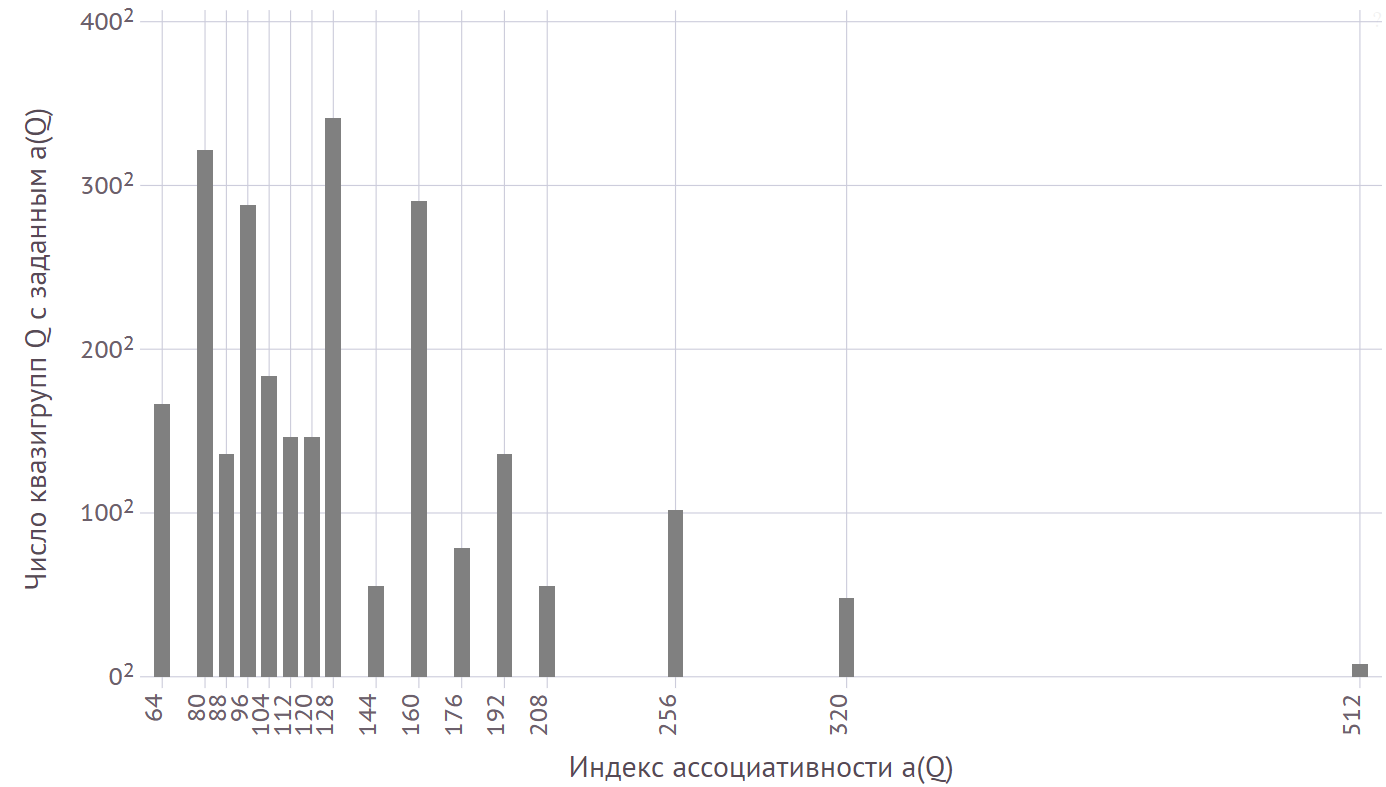
\includegraphics[width=1\linewidth]{histogram.png}
            \caption{Распределение числа квазигрупп с заданным $a(Q)$ для $n = 3$}\label{fig:histogram}
        }
    \end{figure}



    \begin{figure}[ht] % Рисунок
        \centerfloat{
            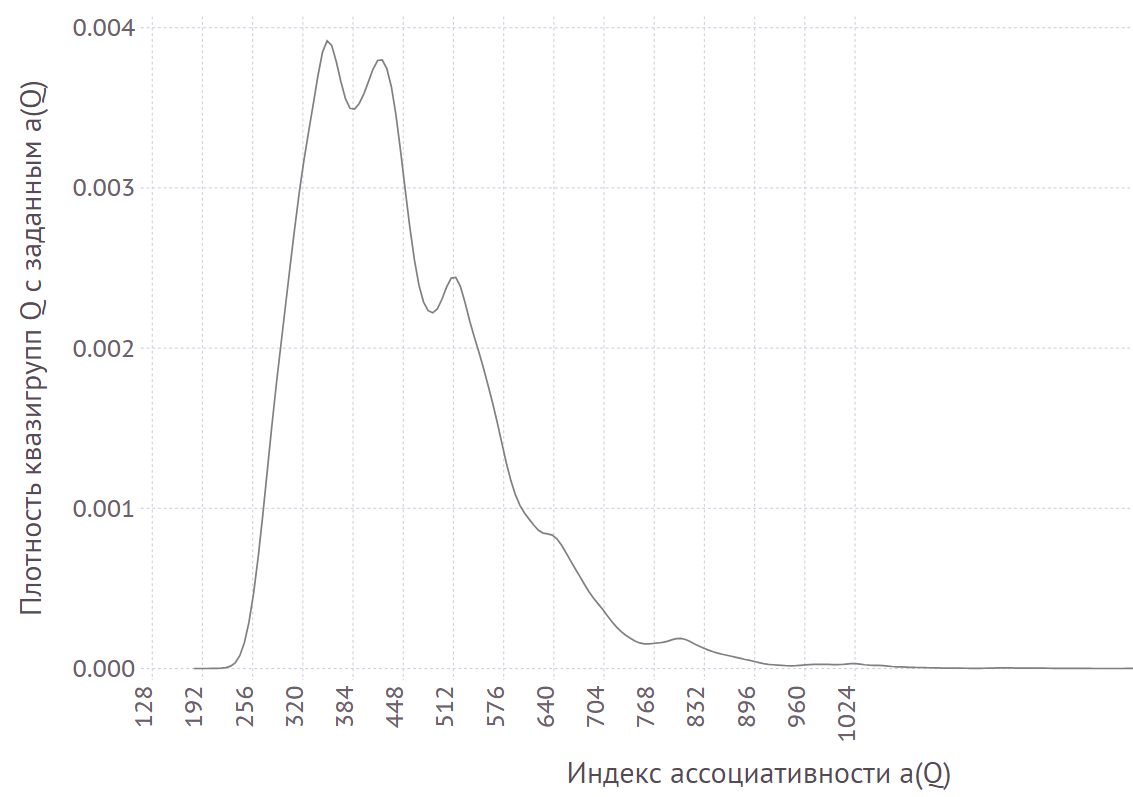
\includegraphics[width=1\linewidth]{density.png}
            \caption{Оценка плотности распределения квазигрупп, построенных по парам правильных булевых семейств, с заданным $a(Q)$ для $n = 4$}\label{fig:density}
        }
    \end{figure}

    Заметим, что при $n = 2$ достигается минимально возможное значение индекса ассоциативности для квазигрупп порядка 4 (а именно 16).
    При~$n \ge 3$ все полученные индексы ассоциативности существенно превышают минимальные теоретически возможные для квазигрупп заданного порядка.
    Отметим также, что во всех исследованных случаях $n = 2, 3, 4$ минимально достижимый индекс ассоциативности у построенных квазигрупп оказался равным квадрату порядка квазигруппы, в связи с чем можно выдвинуть гипотезу, что у квазигрупп, построенным по парам правильных булевых семейств размера $n$, число ассоциативных троек не может быть меньше, чем $2^{2n}$.

    \begin{figure}[ht] % Рисунок
        \centerfloat{
            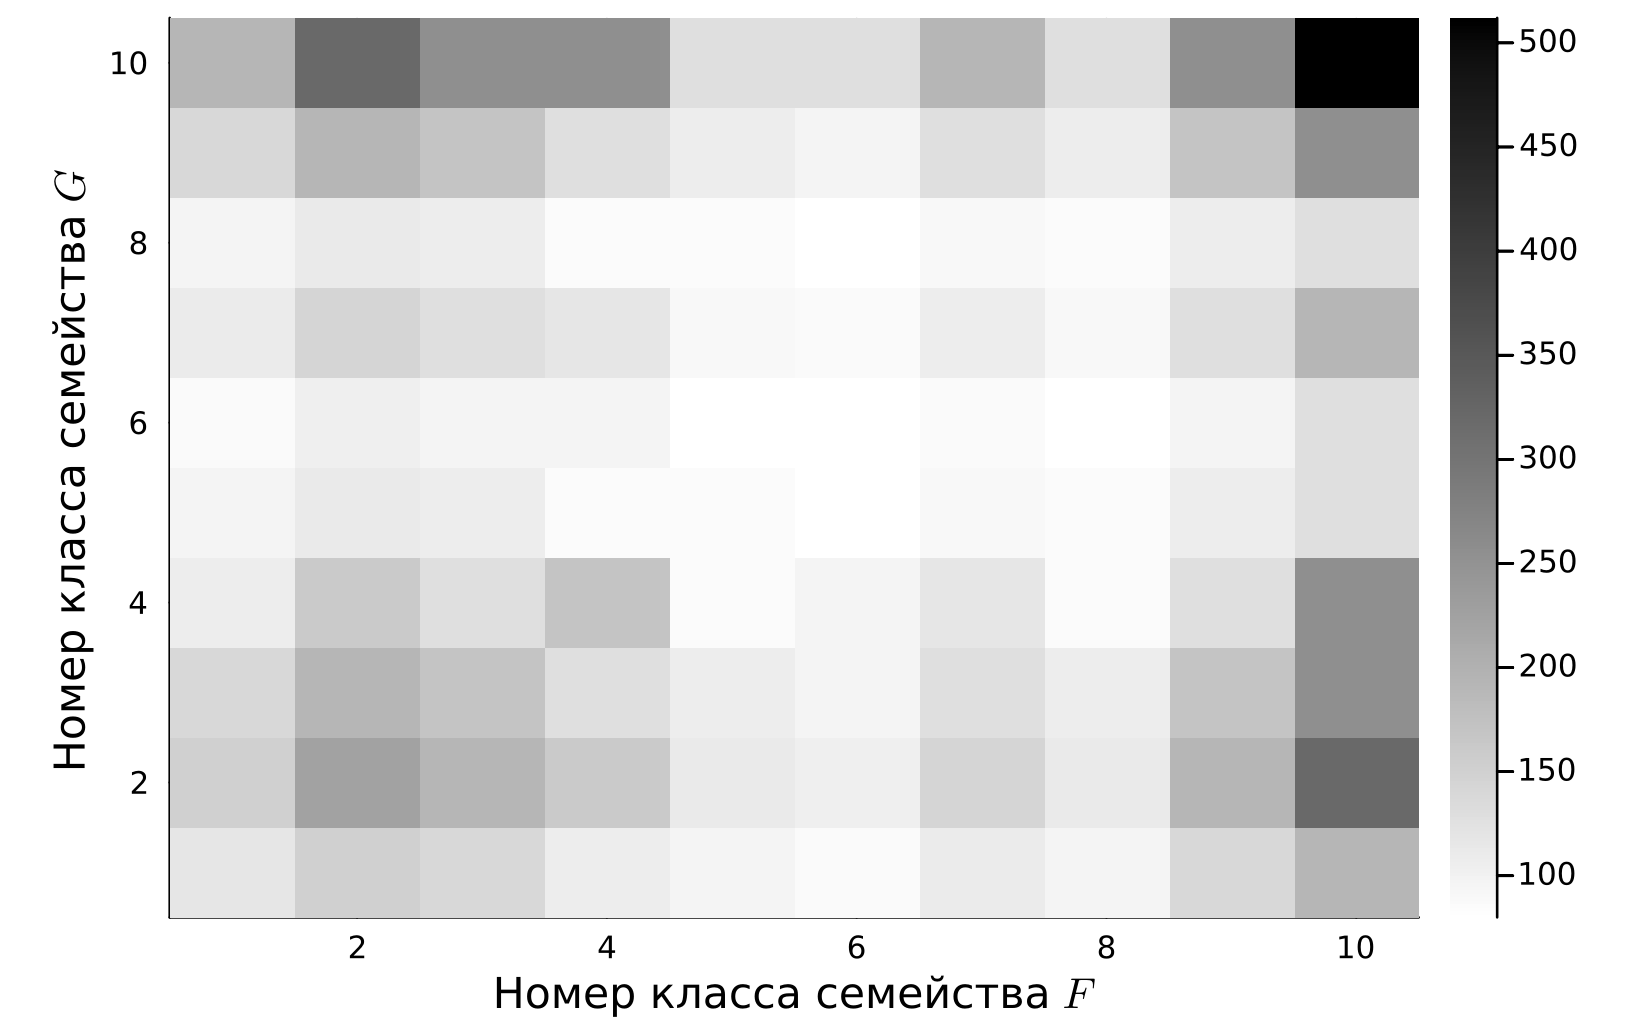
\includegraphics[width=1\linewidth]{heatmap.png}
            \caption{Тепловая карта для среднего индекса ассоциативности, усреднение берется по представителям классов эквивалентности, $n = 3$}\label{fig:heatmap}
        }
    \end{figure}

    Для $n=3$ также был проведен следующий эксперимент.
    Все $744$ правильных семейства были разбиты на $10$ классов эквивалентности относительно изометрий пространства Хэмминга (см. таблицу~\ref{tab:countclasses}).
    Затем для каждой пары классов эквивалентности $(F, G)$ перебирались все пары представителей $\ff \in F$, $\gf \in G$ и вычислялся индекс ассоциативности квазигруппы, порождаемой парой правильных булевых семейств $(\ff, \gf)$, после чего вычислялся \textquote{средний индекс ассоциативности} для пары классов эквивалентности $(F, G)$.
    Результаты эксперимента отображены на рис.~\ref{fig:heatmap}.
    Из приведенной тепловой карты видно, что наиболее неассоциативные квазигруппы порождаются при использовании $6$-го класса эквивалентности, представителем которого является, например, семейство 
    \[
        \left( x_2 x_3, \; x_1 \oplus x_1 x_3, \; x_1 \oplus x_2 \oplus x_1 x_2 \right). 
    \]
    Отметим, что представители указанного класса изучались в разделе~\ref{sec:quadfamily}: было показано, что представители класса имеют полный граф существенной зависимости и являются квадратичным строгого типа $Quad^s_{n-1}Lin^s_{1}$ (см. определение~\ref{def:quadlin}) при четных $n$ и квадратичным строгого типа $Quad^s_{n}Lin^s_{0}$ (сильно квадратичным) при нечетных~$n$ (см. теорему~\ref{thm:strongquad}).



\subsection{Экспериментальное изучение простоты и аффинности}
\label{sec:subquasi_polycomplete}

    Приведем результаты вычислительных экспериментов для квазигрупп, порожденных операцией~(\ref{eq:circ}):
    \begin{equation}
        \xx \circ \yy = \xx + \ff(\xx) + \yy + \gf(\yy),
    \end{equation}
    где в качестве базовой рассматривается группа $\ZZ_2^n$, $\ff$, $\gf$~--- семейства размера $n$ на $\ZZ_2^n$.

    Для $n=2$ существует 12 правильных семейств (см. таблицу~\ref{tab:countfamilies}).
    При этом все 144 квазигруппы, порожденные с помощью конструкции~(\ref{eq:circ}) оказываются аффинными, 32~--- простыми.
    Таким образом, полиномиально полные квазигруппы среди квазигрупп, порожденных конструкцией~(\ref{eq:circ}), для $n=2$ отсутствуют.
    Результаты отображены в таблице~\ref{tab:polycomp2}.

    Для $n=3$ существует 744 правильных семейства и, соответственно, 553536 возможных квазигрупп.
    Среди этих квазигрупп 40000 являются аффинными, 290816~--- простыми, 281600~--- полиномиально полными.
    Результаты отображены в таблице~\ref{tab:polycomp3}.

    \begin{table}[h]
        \begin{center}
            \captionsetup{justification=centering} % выравнивание подписи по-центру
            \caption{\label{tab:polycomp2} Число квазигрупп, построенных с помощью конструкции~(\ref{eq:circ}) с заданными свойствами для $n=2$}
            \begin{tabular}{|c|c|c|}
                \toprule
                Свойства & Афинная & Неаффинная \\
                \midrule
                Не простая & 112 & 0 \\
                \midrule
                Простая & 32 & 0 \\
                \bottomrule
            \end{tabular}
        \end{center}
    \end{table}

    \begin{table}[h]
        \begin{center}
            \captionsetup{justification=centering} % выравнивание подписи по-центру
            \caption{\label{tab:polycomp3} Число квазигрупп, построенных с помощью конструкции~(\ref{eq:circ}) с заданными свойствами для $n=3$}
            \begin{tabular}{|c|c|c|}
                \toprule
                Свойства & Афинная & Неаффинная \\
                \midrule
                Не простая & 30784 & 231936 \\
                \midrule
                Простая & 9216 & 281600 \\
                \bottomrule
            \end{tabular}
        \end{center}
    \end{table}


% \section{Построение правильных семейств}

%     \TODO{расширить: замощения плоскости -- извлечь алгоритм порождения новых правильных семейств?}


\section*{Выводы}

    В настоящей главе были рассмотрены два алгоритма:
    \begin{itemize}
        \item алгоритм шифрования, сохраняющего формат сообщений ($\fpe$-схема), основанный на квазигрупповых сдвигах;
        \item ускоренный алгоритм для задачи распознавания правильности семейства булевых функций.
    \end{itemize}
    Были выделены основные требования к квазигруппам, которые могут использоваться в качестве базовых в предложенной $\fpe$-схеме.
    Также были приведены результаты некоторых статистических и численных экспериментов, в которых изучалось число правильных семейств в различных классах и свойства квазигрупп, порожденных парами правильных семейств булевых функций: индексы ассоциативности, простота и аффинность.
